\section{Четврти домаћи задатак}
\begin{enumerate}[1.]
\item Генерисати по $N=500$ дводимензионалних одбирака из четири класе које ће бити линеарно сепарабилне. Препоручује се да то буду гаусовски расподељени дводимензионални облици. Изабрати једну од метода за кластеризацију (C-mean метод, метод квадратне декомпозиције, метод максималне веродостојности или метод грана и граница) и применити је на формиране узорке класа. Извршити анализу осетљивости изабраног алгоритма на почетну кластеризацију, као и средњи број потребних итерација. Такође извршити анализе случаја када се априорно не познаје број класа.
\item Генерисати по $N=500$ дводимензионалних одбирака из две класе које су нелинеарно сепарабилне. Изабрати једну од метода за кластеризацију које су применљиве за нелинеарно сепарабилне класе (метод квадратне декомпозиције или метод максималне веродостојности) и поновити анализу из претходне тачке.
\end{enumerate}
\subsection{C-Mean алгоритам}
\subsubsection{Генерисање одбирака}
За почетак генерисаћемо одбирке четири дводимензионалних класа чије су функције густине вероватноће у облику  гаусовских расподела:


$$f_1(X) = N(M_{1}, \Sigma_{1}), f_2(X) = N(M_{2}, \Sigma_{2}), f_3(X) = N(M_{3}, \Sigma_{3}),f_4(X) = N(M_{4}, \Sigma_{4})$$
при чему вероватноће, средње вредности и коваријационе матрице имају следеће вредности:
$$ M_{1} = \begin{bmatrix}
   -4\\
   -4
\end{bmatrix}, 
 M_{2} = \begin{bmatrix}
   4\\
   4
\end{bmatrix}, 
 M_{3} = \begin{bmatrix}
   4\\
   -4
\end{bmatrix}, 
 M_{1} = \begin{bmatrix}
   -4\\
   4
\end{bmatrix}, 
 M_{4} = \begin{bmatrix}
   -4\\
   4
\end{bmatrix}, 
$$				
$$S_{1} = \begin{bmatrix}
				   1,5 & 1\\
				   1 & 2,5
				\end{bmatrix},
S_{2} = \begin{bmatrix}
	2 & 1\\
	1 & 2
\end{bmatrix},
S_{1} = \begin{bmatrix}
	1,5 & -1\\
	-1 & 1,5
\end{bmatrix},
S_{1} = \begin{bmatrix}
	2 & -1\\
	-1 & 2
\end{bmatrix}$$

\renewcommand{\lstlistingname}{Одсечак кода}%
Добијају се 4 класе одбирака као на слици \ref{fig:Odbirci}
\begin{figure}[htb!]
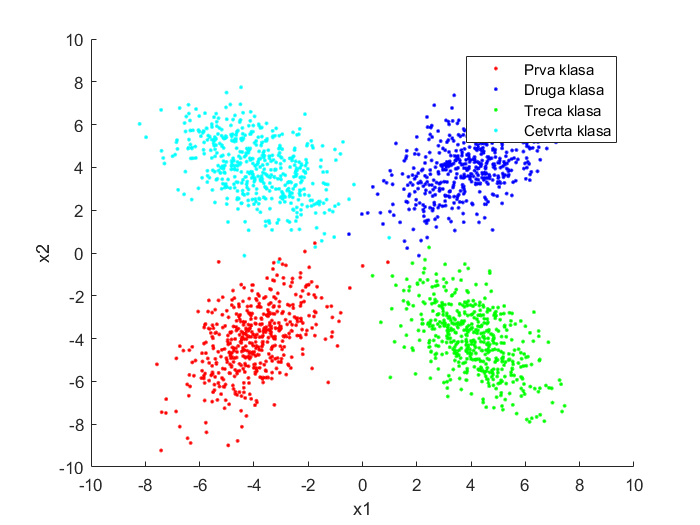
\includegraphics[scale=.8]{pictures/4/Odbirci}
\caption{Одбирци}\label{fig:Odbirci}
\end{figure}

\subsubsection{Алгоритам}
Кластеризацију над датим скупомо података ћемо извршити уз помоћ C-mean алгоритма. Једна од предности ове методе су њена једноставност, могућност стохастичке почетне кластеризације. Међутим, има и одређених ограничења. Кластери су поељени део по део линеарним линијама, што ограничава примену ове методе на линеарно сепарабилне класе. Такође, захтева априорно знање о броју кластера и не гарантује глобалну конвергенцију.

Одсечак кода \ref{fun:cMean} имплементира c-Mean алгоритам.


\begin{lstlisting}[caption={C-Mean функција},label={fun:cMean}]
function [num_it, critFun] = cMean(X1, X2, X3, X4, num_points, num_classes, apPer, drawFigure)

chunkRand = floor((1 - apPer) * num_points);
chunkApp = num_points - chunkRand;

Z = [X1(1 : chunkRand, :); X2(1 : chunkRand, :); ...
     X3(1 : chunkRand, :); X4(1 : chunkRand, :);];

num_points_all = 4 * chunkRand;

idx = randperm(num_points_all);
chunk_size = floor(num_points_all / num_classes);

Y1 = Z(idx(1 : chunk_size), :);
Y1App = X1(chunkRand + 1 : num_points, :);
Y1 = [Y1App; Y1];
Y2 = Z(idx(chunk_size + 1:2 * chunk_size), :);
Y2App = X2(chunkRand + 1 : num_points, :);
Y2 = [Y2App; Y2];
Y3 = [];
Y3App = [];
Y4 =[];
Y4App = [];
Y5 =[];
Y5App = [];
if (num_classes > 2)
    Y3 = Z(idx(2 * chunk_size + 1:3 * chunk_size), :);
    Y3App = X3(chunkRand + 1 : num_points, :);
    Y3 = [Y3App; Y3];
end 
if (num_classes > 3)
    Y4 = Z(idx(3 * chunk_size + 1:4 * chunk_size), :);
    Y4App = X4(chunkRand + 1 : num_points, :);
    Y4 = [Y4App; Y4];
end
if (num_classes > 4)
    Y5 = Z(idx(4 * chunk_size + 1:5 * chunk_size), :);
end
run = 1;

it = 0;

while (run && it < 50)
    it = it + 1;
    M1 = mean(Y1);
    M2 = mean(Y2);
    M3 = mean(Y3);
    M4 = mean(Y4);
    M5 = mean(Y5);
    
    if (size(M1, 2) == 1)
        M1 = [realmax realmax];
    end 
    if (size(M2, 2) == 1)
        M2 = [realmax realmax];
    end 
    if (size(M3, 2) == 1)
        M3 = [realmax realmax];
    end 
    if (size(M4, 2) == 1)
        M4 = [realmax realmax];
    end 
    if (size(M5, 2) == 1)
        M5 = [realmax realmax];
    end 
    clear X1 X2 X3 X4;
    
    M = [M1; M2; M3; M4; M5];
    
    [X11, X21, X31, X41, X51, changed1] = reCluster(Y1(chunkApp + 1: end, :), M, 1);
    [X12, X22, X32, X42, X52, changed2] = reCluster(Y2(chunkApp + 1: end, :), M, 2);
    [X13, X23, X33, X43, X53, changed3] = reCluster(Y3(chunkApp + 1: end, :), M, 3);
    [X14, X24, X34, X44, X54, changed4] = reCluster(Y4(chunkApp + 1: end, :), M, 4);
    [X15, X25, X35, X45, X55, changed5] = reCluster(Y5(chunkApp + 1: end, :), M, 5);
    run = changed1 | changed2 | changed3 | changed4 | changed5;
    Y1 = [Y1App; X11; X12; X13; X14; X15];
    Y2 = [Y2App; X21; X22; X23; X24; X25];
    Y3 = [Y3App; X31; X32; X33; X34; X35];
    Y4 = [Y4App; X41; X42; X43; X44; X45];
    Y5 = [Y5App; X51; X52; X53; X54; X55];
end

num_it = it;
\end{lstlisting}

 На почетку алгоритма имамо насумично кластеризовање података.  На сликама  \ref{pic:cMean2Init}, \ref{pic:cMean3Init}, \ref{pic:cMean4Init}, \ref{pic:cMean5Init} видимо почетне кластеризације за различит број почетних класа. 
 
\begin{figure}[htb!]\caption{Иницијална кластеризација}
\begin{subfigure}{.6\textwidth}
\centering
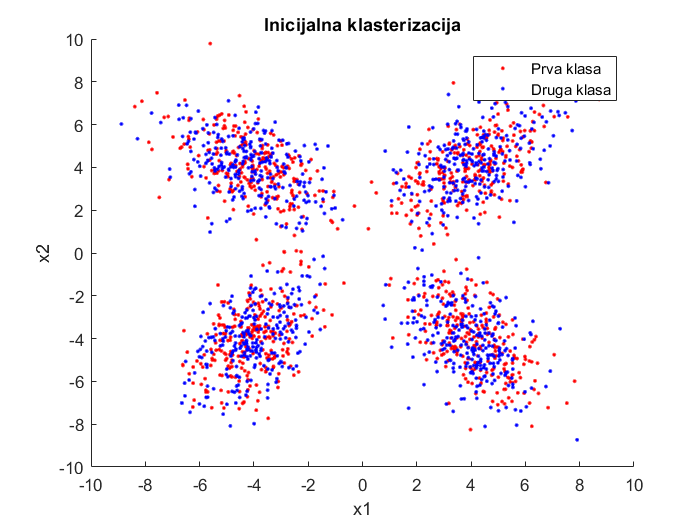
\includegraphics[width=1\textwidth]{pictures/4/CMean2Init}
\caption{Случај кад је $L=2$}\label{pic:cMean2Init}
\end{subfigure}
\begin{subfigure}{.55\textwidth}
\centering
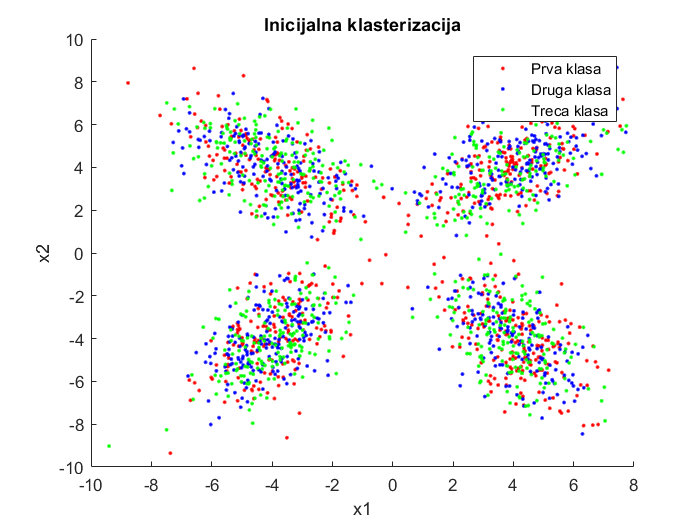
\includegraphics[width=1\linewidth]{pictures/4/CMean3Init}
\caption{Случај кад је $L=3$}\label{pic:cMean3Init}
\end{subfigure}
\bigskip
\begin{subfigure}{.55\textwidth}
\centering
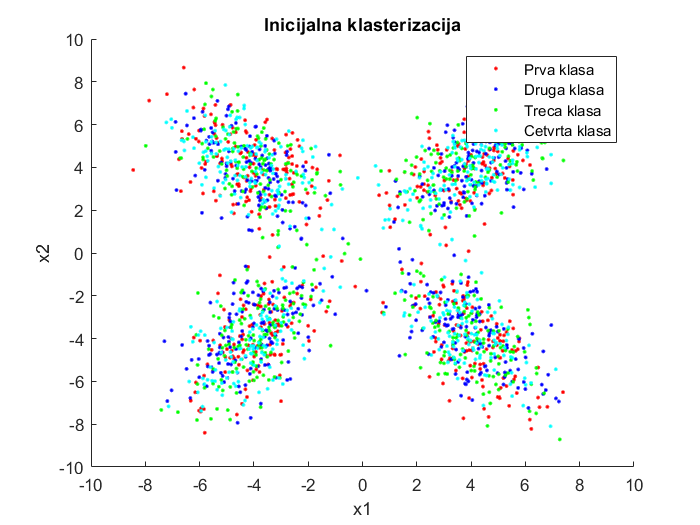
\includegraphics[width=1\linewidth]{pictures/4/CMean4Init}
\caption{Случај кад је $L=4$}\label{pic:cMean4Init}
\end{subfigure}
\begin{subfigure}{.55\textwidth}
\centering
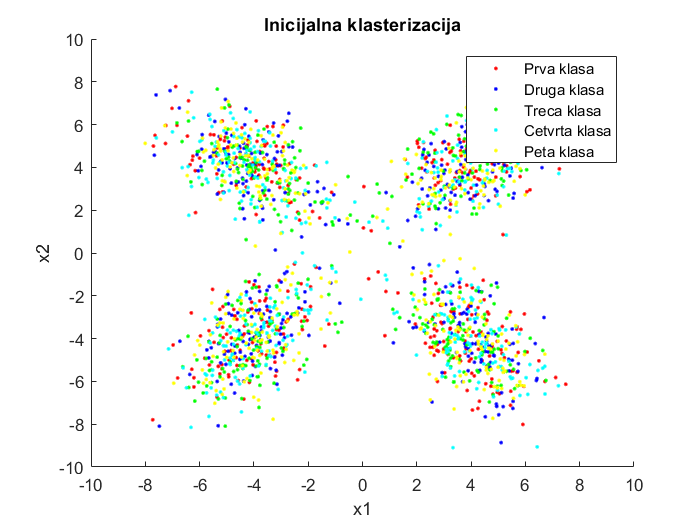
\includegraphics[width=1\linewidth]{pictures/4/CMean5Init}
\caption{Случај кад је $L=5$}\label{pic:cMean5Init}
\end{subfigure}
\end{figure}

Критеријум минимизује критеријумску функцију:
$$J=\frac{1}{N}\sum_{r=1}^L\sum_{j=1}^{N_r}||X_j^{(r)} - M_r||^2$$
где је $N$-укупан број одбирака, $L$-укупан број кластера, $M_r$-вектор средње вредности $r$-тог кластера, $N_r$-број елемената у $r$-том кластеру. С обзиром да критеријум минимизује средње квадратно одступање од центара кластера, закључује се да ће се сваки одбирак придружити најближем центру кластера. Међутим, овде се може закључити да C-mean узима у обзир само математичко очекивање, али не и коваријационе матрице одбирака. Сређивање израза добија се да је правило одлучивања:
$$||X_i - M_t(l)|| = \min_{1 \leq j \leq L}||X_i - M_j(l)|| \implies X_i \in \omega_t$$
Дакле прво се обави рекласификација, потом поново се израчуна $M_j(l)$ и то се извршава док има промене изгледа кластера. Кад нема завршава се.  Одсечци кода \ref{fun:cMeanClusterFind} и \ref{fun:cMeanCluster} су функције које имплементирају логику налажења минималне вредности критеријумске функције.

\begin{lstlisting}[caption={Функција налажења кластера за дате одбирке},label={fun:cMeanCluster}]
function [X1, X2, X3, X4, X5, changed] = reCluster(Y,M, curId)
changed = 0;
X1 = [];
X2 = [];
X3 = [];
X4 = [];
X5 = [];
 for i = 1 : size(Y, 1)
        clusterId = findClosesestDist(Y(i, :), M);
        if clusterId ~= curId
            changed = 1;
        end
        switch clusterId
            case 1
                X1 = [X1; Y(i, :)];
            case 2
                X2 = [X2; Y(i, :)];
             case 3
                X3 = [X3; Y(i, :)];
             case 4
                X4 = [X4; Y(i, :)];
            case 5
                X5 = [X5;  Y(i, :)];
        end
    end
end
\end{lstlisting}

\begin{lstlisting}[caption={Функција налажења кластера за дати одбирак},label={fun:cMeanClusterFind}]
function [clusterId] = findClosesestDist(elem, center)
for i = 1 : distLen
    curCenter = center(i, :);
    curDist = sqrt(sum((elem - curCenter).^2));
    if (curDist < distMin)
        distMin = curDist;
        distMinIdx = i;
    end
end
clusterId = distMinIdx;
\end{lstlisting}


Крајњи резултат извршавања се може видети на сликама  \ref{pic:cMean2Final}, \ref{pic:cMean3Final}, \ref{pic:cMean4Final}, \ref{pic:cMean5Final}.	

\begin{figure}[htb!]\caption{Крајња кластеризација}
\begin{subfigure}{.6\textwidth}
\centering
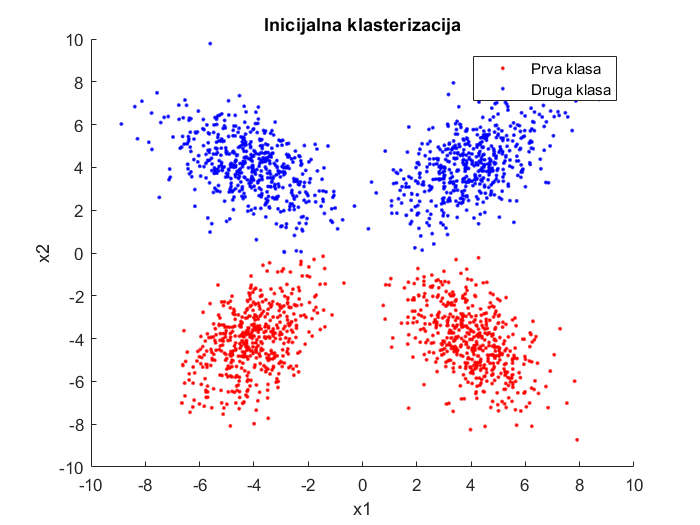
\includegraphics[width=1\textwidth]{pictures/4/CMean2Final}
\caption{Случај кад је $L=2$}\label{pic:cMean2Final}
\end{subfigure}
\begin{subfigure}{.55\textwidth}
\centering
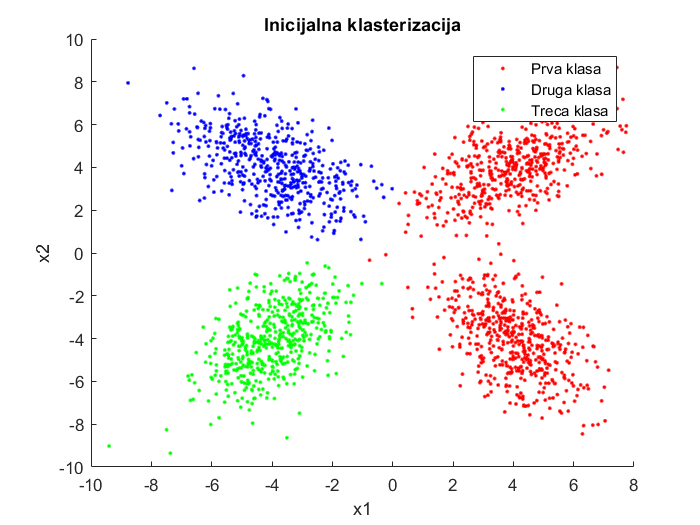
\includegraphics[width=1\linewidth]{pictures/4/CMean3Final}
\caption{Случај кад је $L=3$}\label{pic:cMean3Final}
\end{subfigure}
\bigskip
\begin{subfigure}{.55\textwidth}
\centering
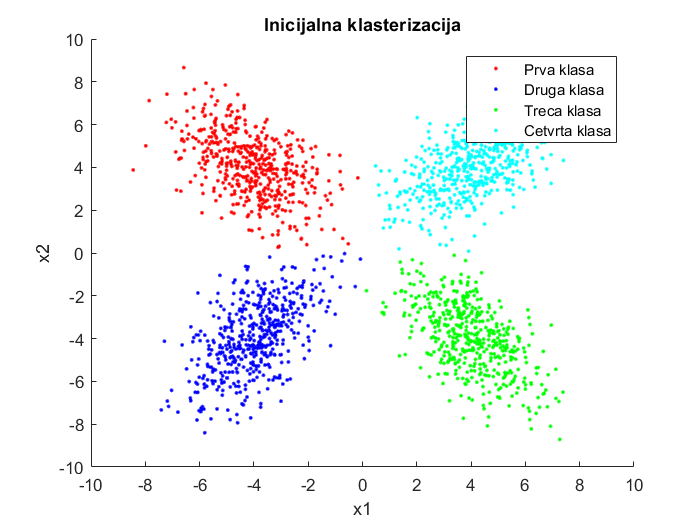
\includegraphics[width=1\linewidth]{pictures/4/CMean4Final}
\caption{Случај кад је $L=4$}\label{pic:cMean4Final}
\end{subfigure}
\begin{subfigure}{.55\textwidth}
\centering
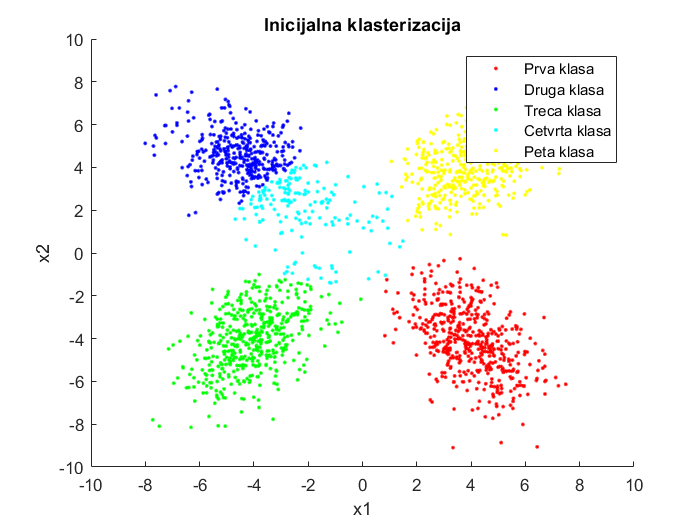
\includegraphics[width=1\linewidth]{pictures/4/CMean5Final}
\caption{Случај кад је $L=5$}\label{pic:cMean5Final}
\end{subfigure}
\end{figure}
\subsubsection{Анализа резултата алгоритма}
Алгоритам није превише осетљив на почетну кластеризацију, али не гарантује да ће се достићи оптимална кластеризација (у зависности од почетне расподеле у случају $L=4$ добије се изглед као \ref{pic:cMean3Final}). Просечан број итерација за иницијално претпостављене величине кластера $L=2, L=3, L=4,L=5$ варира, али усредњене вредности су редом $3,7 ; 5,93; 6,42; 9,13$. Ово је и у неку руку јасно јер су ове 4 класе на неки начин подељена на 2 скупа одбирака, односно 4, стога просечан број итерација расте драстично са случаја $L=2$ на случај $L=3$ и са $L=4$ на $L=5$, док са $L=3$ на $L=4$ не расте.  Ако је међутим познат број неких тачака које припадају одређеним кластерима, ово може да убрза рад алгоритма значајно. У случају $L=4$ добија се да за априорно вероватноћу познавања броја одбирака одређеног кластера $0,1$ просечан број одбирака је $3,7$ а за случај $0,25$ спада на 3, а за $0,5$ чак je спао на $2,3$, што је и логично јер су кластери већ у неку руку одређени. 

Уколико априорно није познат број кластера неопходно је одрадит минимизацију коришћењем неког критеријума. Мало измењена верзија Акаикевог критеријума $AIC(L) =J(L) + ln(L)$ где је $J(L)$ минимизирана критеријумска функција за конкретан број кластера. Редом, за различит број класа 2, 3, 4, 5 су добијене $20, 10;12.8;5,194;5,68$.  Што и каже оно што видимо на слици, да постоје 4 класе.

\subsection{Метод квадратне декомпозиције}
\subsubsection{Генерисање одбирака}
За почетак генерисаћемо одбирке двеју дводимензионалних класа чије су функције густине вероватноће у облику бимодалних гаусовских расподела:


$$f_1(X) = P_{11} N(M_{11}, \Sigma_{11}) + P_{12} N(M_{12}, \Sigma_{12})$$
$$f_2(X) = P_{21} N(M_{21}, \Sigma_{21}) + P_{22} N(M_{22}, \Sigma_{22}),$$
при чему вероватноће, средње вредности и коваријационе матрице имају следеће вредности:
$$P_{11} = 0,6,  M_{11} = \begin{bmatrix}
   1,5\\
   -4,5
\end{bmatrix}, 
S_{11} = \begin{bmatrix}
				   3,5 & -1\\
				   -1 & 2,2
				\end{bmatrix},
P_{12} = 0,4,  M_{12} = \begin{bmatrix}
										   -0,5\\
										   0,5
										\end{bmatrix}, 
S_{12} = \begin{bmatrix}
				   1,3 & 0,9\\
			   	0,9 &  2
				\end{bmatrix}
$$				
$$P_{21} = 0,45,  M_{21} = \begin{bmatrix}
   12\\
   -3,5
\end{bmatrix}, 
S_{21} = \begin{bmatrix}
				   1,5 & 1,1\\
				   1,1 & 1,5
				\end{bmatrix},
P_{22} = 0,55,  M_{22} = \begin{bmatrix}
										   -10\\
										   2
										\end{bmatrix}, 
S_{22} = \begin{bmatrix}
				   3 & -0,8\\
			   	-0,8 &  3
				\end{bmatrix}
$$

Добијају се 2 класе одбирака као на слици \ref{fig:OdbirciQuad}.

\begin{figure}[htb!]
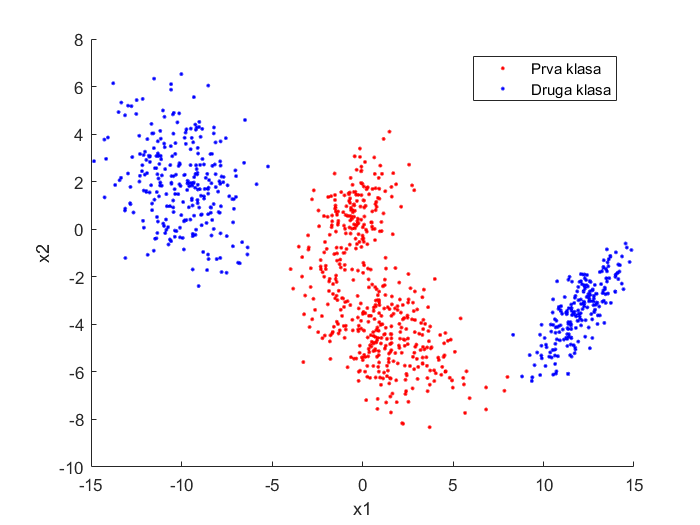
\includegraphics[scale=.8]{pictures/4/OdbirciQuad}
\caption{Одбирци}\label{fig:OdbirciQuad}
\end{figure}

\subsubsection{Алгоритам}
Овај метод је сложенији и захтевнији за израчунавање. Али његова предност је што границе изђему кластера не морају да буду само линеарне, него су квадратне криве. Стога се он употребљава кад је потребна кластеризација нелинеарлно сепарабилних класа. 
Одсечак кода представља \ref{fun:quadr} имплементацију алгоритма.

На почетку се изабере иницијална кластеризација $\Omega(0)$ И на основу ње процене априорне вероватноће појава $P_i(0)$ вектори средњих вредности класа $M_i(0)$, Као и коваријационе матриц $\Sigma_i(0)$. У свакој итерацији одбирак $X_j$ се придрућује класи $t$ за коју је дати израз најмањи:
$$(X_j - M_t(l))^T\Sigma_t^{-1}(l)(X_j-M_t(l)) + ln|\Sigma_t(l)| - ln(P_t(l))$$
Логика испитивања минималне вредност критеријумске функције имплементирана је функцијом чији је одсечак кода је  \ref{fun:reclusterQuadr} и функцијом чији одсечак кода је \ref{fun:reclusterQuadSearch} .

\begin{lstlisting}[caption={Метод квадратне декомпозиције},label={fun:quadr}]
function [num_it, critFun] = quadratic(X1, X2, num_points, num_classes, apPer, drawFigure)

chunkRand = floor((1 - apPer) * num_points);
chunkApp = num_points - chunkRand;

Z = [X1(1 : chunkRand, :); X2(1 : chunkRand, :);];

num_points_all = 2 * chunkRand;

idx = randperm(num_points_all);
chunk_size = floor(num_points_all / num_classes);

Y1 = Z(idx(1 : chunk_size), :);
Y1App = X1(chunkRand + 1 : num_points, :);
Y1 = [Y1App; Y1];
Y2 = Z(idx(chunk_size + 1:2 * chunk_size), :);
Y2App = X2(chunkRand + 1 : num_points, :);
Y2 = [Y2App; Y2];
Y3 = [];
Y3App = [];
Y4 =[];
Y4App = [];
Y5 =[];
Y5App = [];
if (num_classes > 2)
    Y3 = Z(idx(2 * chunk_size + 1:3 * chunk_size), :);
end 
if (num_classes > 3)
    Y4 = Z(idx(3 * chunk_size + 1:4 * chunk_size), :);
end
if (num_classes > 4)
    Y5 = Z(idx(4 * chunk_size + 1:5 * chunk_size), :);
end

run = 1;

it = 0;

while (run && it < 50)
    it = it + 1;
    M1 = mean(Y1);
    M2 = mean(Y2);
    M3 = mean(Y3);
    M4 = mean(Y4);
    M5 = mean(Y5);
    
    S1 = cov(Y1);
    S2 = cov(Y2);
    S3 = cov(Y3);
    S4 = cov(Y4);
    S5 = cov(Y5);
    P1 = size(Y1, 1) / (2 * num_points);
    P2 = size(Y2, 1) / (2 * num_points);
    P3 = size(Y3, 1) / (2 * num_points);
    P4 = size(Y4, 1) / (2 * num_points);
    P5 = size(Y5, 1) / (2 * num_points);
    
    if (size(M1, 2) == 1)
        M1 = [realmax realmax];
        S1 = [realmax realmax; realmax realmax];
    end 
    if (size(M2, 2) == 1)
        M2 = [realmax realmax];
        S2 = [realmax realmax; realmax realmax];
    end 
    if (size(M3, 2) == 1)
        M3 = [realmax realmax];
        S3 = [realmax realmax; realmax realmax];
    end 
    if (size(M4, 2) == 1)
        M4 = [realmax realmax];
        S4 = [realmax realmax; realmax realmax];
    end 
    if (size(M5, 2) == 1)
        M5 = [realmax realmax];
        S5 = [realmax realmax; realmax realmax];
    end 
    clear X1 X2 X3 X4;
    
    M = [M1; M2; M3; M4; M5];
    S = [S1; S2; S3; S4; S5];
    P = [P1; P2; P3; P4; P5];
    
    [X11, X21, X31, X41, X51, changed1] = reClusterQuadr(Y1(chunkApp + 1: end, :), M, S, P, 1);
    [X12, X22, X32, X42, X52, changed2] = reClusterQuadr(Y2(chunkApp + 1: end, :), M, S, P, 2);
    [X13, X23, X33, X43, X53, changed3] = reClusterQuadr(Y3(chunkApp + 1: end, :), M, S, P, 3);
    [X14, X24, X34, X44, X54, changed4] = reClusterQuadr(Y4(chunkApp + 1: end, :), M, S, P, 4);
    [X15, X25, X35, X45, X55, changed5] = reClusterQuadr(Y5(chunkApp + 1: end, :), M, S, P, 5);
    run = changed1 | changed2 | changed3 | changed4 | changed5;
    Y1 = [Y1App; X11; X12; X13; X14; X15];
    Y2 = [Y2App; X21; X22; X23; X24; X25];
    Y3 = [Y3App; X31; X32; X33; X34; X35];
    Y4 = [Y4App; X41; X42; X43; X44; X45];
    Y5 = [Y5App; X51; X52; X53; X54; X55];
end

num_it = it;
\end{lstlisting}

\begin{lstlisting}[caption={Функција проналажења одговарајућег кластера},label={fun:reclusterQuadr}]
function [X1, X2, X3, X4, X5, changed] = reClusterQuadr(Y, M, S, P, curId)
changed = 0;
X1 = [];
X2 = [];
X3 = [];
X4 = [];
X5 = [];
 for i = 1 : size(Y, 1)
        clusterId = findClosesestDistQuadr(Y(i, :), M, S, P);
        if clusterId ~= curId
            changed = 1;
        end
        switch clusterId
            case 1
                X1 = [X1; Y(i, :)];
            case 2
                X2 = [X2; Y(i, :)];
             case 3
                X3 = [X3; Y(i, :)];
             case 4
                X4 = [X4; Y(i, :)];
            case 5
                X5 = [X5;  Y(i, :)];
        end
    end
end
\end{lstlisting}

\begin{lstlisting}[caption={Функција проналажења одговарајућег кластера},label={fun:reclusterQuadSearch}]
function [clusterId] = findClosesestDistQuadr(elem, M, S, P)
distLen = size(M, 1);
distMinIdx = 0;
distMin = realmax;
for i = 1 : distLen
    curM = M(i, :);
    curS = S(2 * i - 1 : 2 * i, :);
    curP = P(i, :);
    if (S(2*i - 1, 1) > 10000)
        j = realmax;
    else
        j = (elem - curM) * inv(curS) * (elem - curM)' + log(det(curS)) - log(curP);
    end
    if (j < distMin)
        distMin = j;
        distMinIdx = i;
    end
end
clusterId = distMinIdx;
\end{lstlisting}

 На почетку алгоритма имамо насумично кластеризовање података.  На сликама  \ref{pic:Quad2Init}, \ref{pic:Quad3Init}, \ref{pic:Quad4Init}, \ref{pic:Quad5Init} видимо почетне кластеризације за различит број почетних класа. 
\begin{figure}[htb!]\caption{Иницијална кластеризација}
\begin{subfigure}{.6\textwidth}
\centering
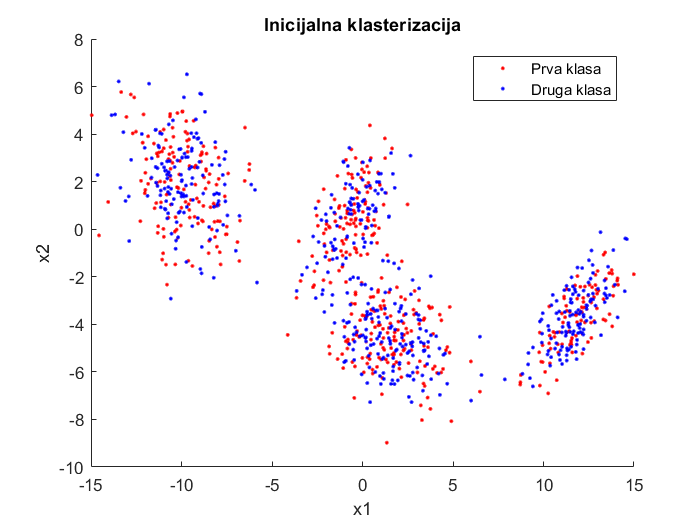
\includegraphics[width=1\textwidth]{pictures/4/Quad2Init}
\caption{Случај кад је $L=2$}\label{pic:Quad2Init}
\end{subfigure}
\begin{subfigure}{.55\textwidth}
\centering
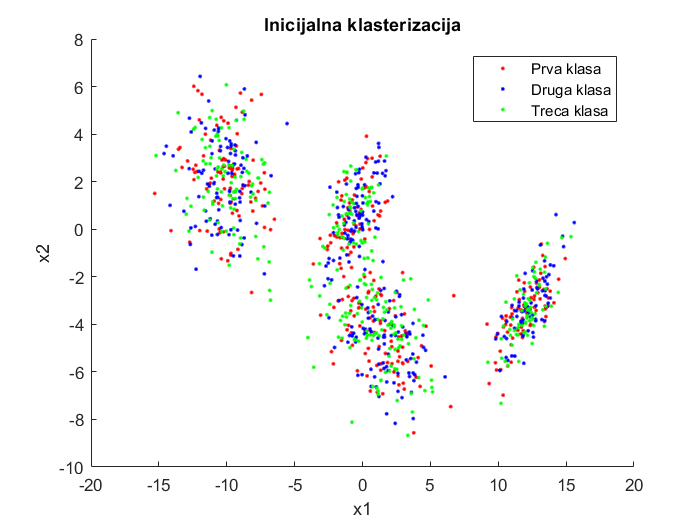
\includegraphics[width=1\linewidth]{pictures/4/Quad3Init}
\caption{Случај кад је $L=3$}\label{pic:Quad3Init}
\end{subfigure}
\bigskip
\begin{subfigure}{.55\textwidth}
\centering
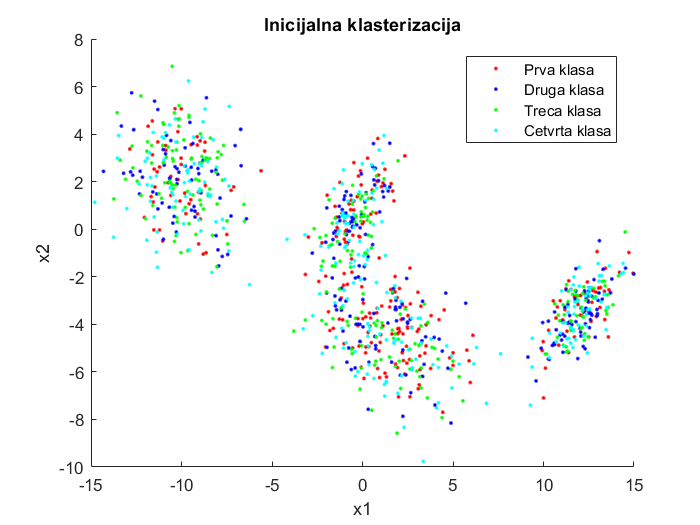
\includegraphics[width=1\linewidth]{pictures/4/Quad4Init}
\caption{Случај кад је $L=4$}\label{pic:Quad4Init}
\end{subfigure}
\begin{subfigure}{.55\textwidth}
\centering
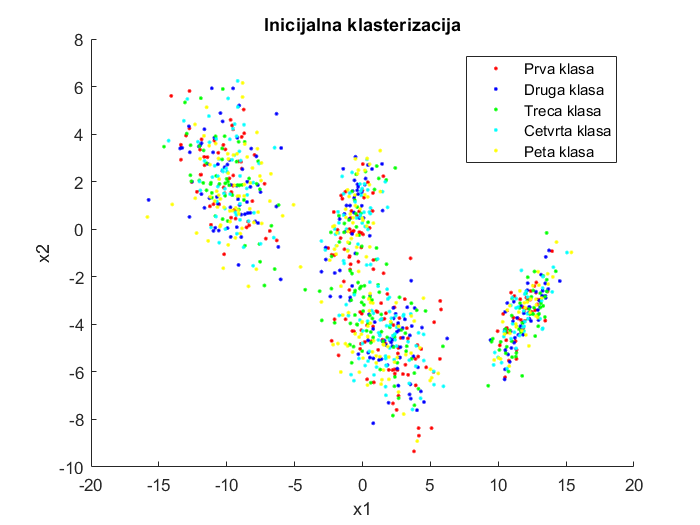
\includegraphics[width=1\linewidth]{pictures/4/Quad5Init}
\caption{Случај кад је $L=5$}\label{pic:Quad5Init}
\end{subfigure}
\end{figure}

Крајњи резултат извршавања се може видети на сликама  \ref{pic:Quad2Final}, \ref{pic:Quad3Final}, \ref{pic:Quad4Final}, \ref{pic:Quad5Final}.	 Дакле алгоритам уопште не кластеризује добро.
\begin{figure}[htb!]\caption{Крајња кластеризација}
\begin{subfigure}{.6\textwidth}
\centering
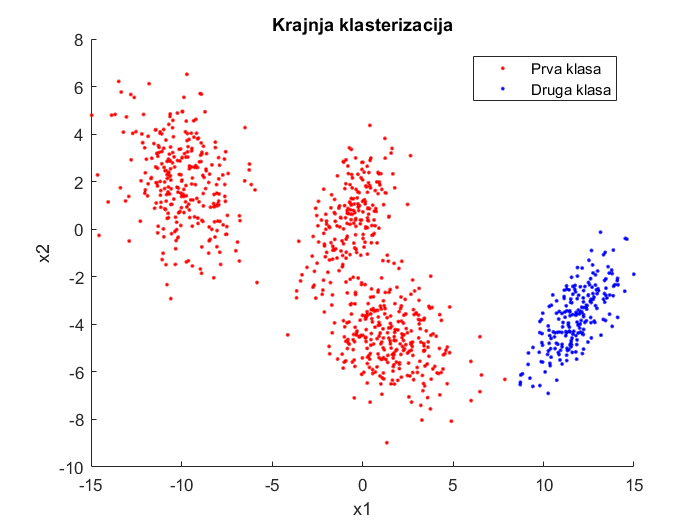
\includegraphics[width=1\textwidth]{pictures/4/Quad2Final}
\caption{Случај кад је $L=2$}\label{pic:Quad2Final}
\end{subfigure}
\begin{subfigure}{.55\textwidth}
\centering
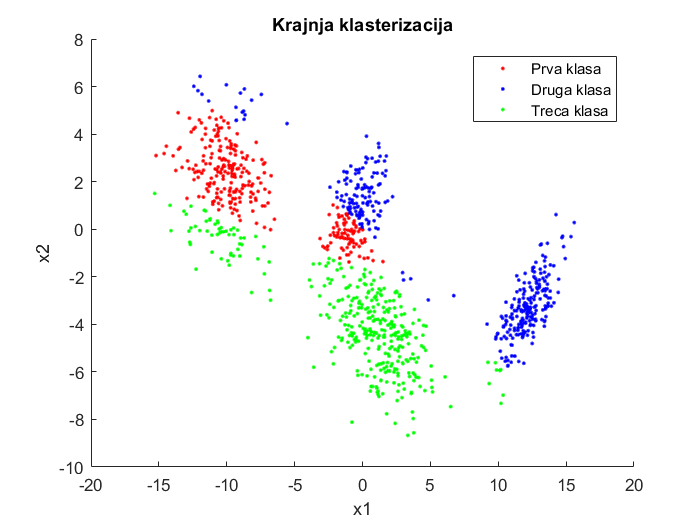
\includegraphics[width=1\linewidth]{pictures/4/Quad3Final}
\caption{Случај кад је $L=3$}\label{pic:Quad3Final}
\end{subfigure}
\bigskip
\begin{subfigure}{.55\textwidth}
\centering
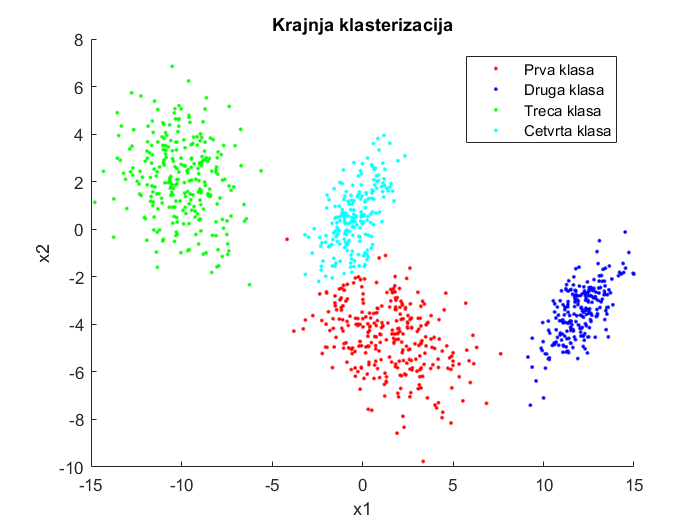
\includegraphics[width=1\linewidth]{pictures/4/Quad4Final}
\caption{Случај кад је $L=4$}\label{pic:Quad4Final}
\end{subfigure}
\begin{subfigure}{.55\textwidth}
\centering
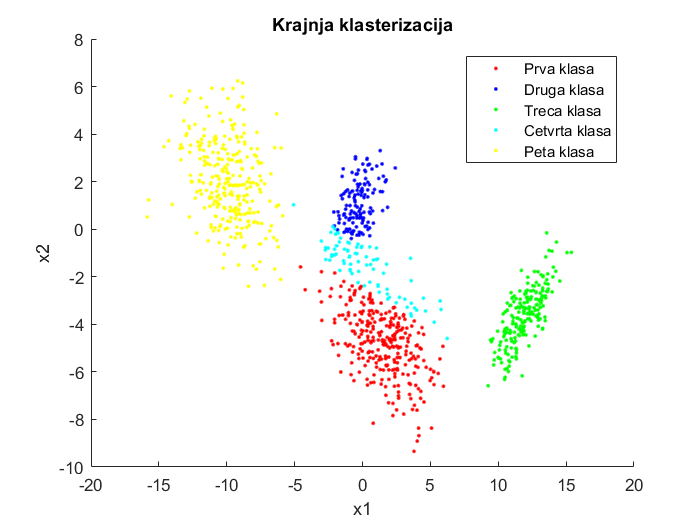
\includegraphics[width=1\linewidth]{pictures/4/Quad5Final}
\caption{Случај кад је $L=5$}\label{pic:Quad5Final}
\end{subfigure}
\end{figure}


\subsubsection{Анализа резултата}
Алгоритам је осетљив на почетну кластеризацију, и не гарантује да ће се достићи оптимална кластеризација. Просечан број итерација за иницијално претпостављене величине кластера $L=2, L=3, L=4,L=5$ варира, али усредњене вредности су редом $10.2 ; 17.9; 20.4; 20.1$. Ово је и у неку руку јасно јер су ове 2 класе на неки начин подељена на 2 скупа одбирака, стога просечан број итерација расте драстично са случаја $L=2$ на случај $L=3$ и релативно,  драстично са $L=3$ на $L=4$ док са $L=4$ на $L=5$ чак и опада.  Ако је међутим познат број неких тачака које припадају одређеним кластерима, ово може да убрза рад алгоритма значајно и да се постигне тачност. У случају $L=4$ добија се да за априорно вероватноћу познавања броја одбирака одређеног кластера $0,1$ просечан број одбирака је $7,1$ а за случај $0,25$ спада на $6$а за $0,5$ чак je спао на $4,6$. Такође, са порастом априорне вероватноће познавања броја одбирака одређеног кластера, добија се пуно већа тачност, што за вероватноће $0,15$ и $0,25$ можемо да видимо на сликама \ref{pic:Quad15Final} и \ref{pic:Quad20Final} да је релативно добро одредио кластере.

Уколико априорно није познат број кластера неопходно је одрадит минимизацију коришћењем неког критеријума. Мало измењена верзија Акаикевог критеријума $AIC(L) =J(L) +3 ln(L)$ где је $J(L)$ минимизирана критеријумска функција за конкретан број кластера. Редом, за различит број класа 2, 3, 4, 5 су добијене $8,778;8,76;8,62;9,16$.  Што и каже оно што видимо на слици, да постоје 2 класе, али подједнаке шансе постоје и да постоје 3 и 4.

\begin{figure}[htb!]\caption{Крајња кластеризација}
\begin{subfigure}{.6\textwidth}
\centering
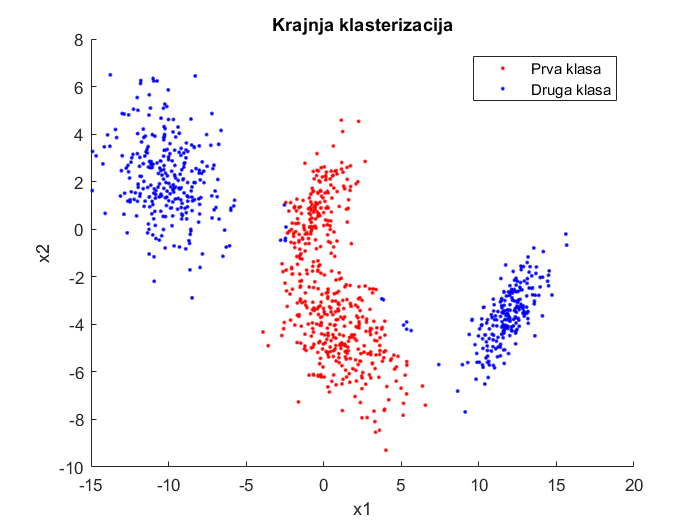
\includegraphics[width=1\textwidth]{pictures/4/QuadrFinal15}
\caption{Случај кад је априорна вероватноћа 15\%}\label{pic:Quad15Final}
\end{subfigure}
\begin{subfigure}{.55\textwidth}
\centering
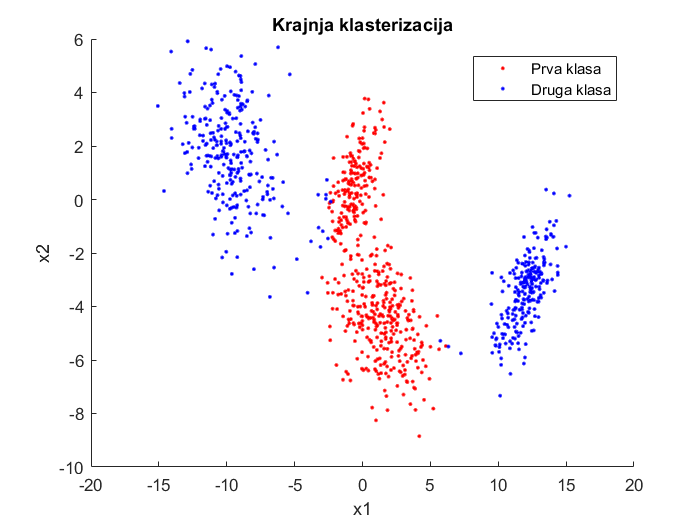
\includegraphics[width=1\linewidth]{pictures/4/QuadrFinal25}
\caption{Случај кад је априорна вероватноћа 25\%}\label{pic:Quad20Final}
\end{subfigure}

\end{figure}


